%
% Copyright (c) 2009  Betti "Osterholz
%
% Permission is granted to copy, distribute and/or modify this document
% under the terms of the GNU Free Documentation License, Version 1.2 or
% any later version published by the Free Software Foundation;
% with no Invariant Sections, no Front-Cover Texts, and no Back-Cover Texts.
%
% A copy of the license is included in the file ``fdl.tex'' .
%
%History:
% 19.12.2009  Oesterhol  erstellt

%path for pictures
\graphicspath{{./sonstiges/}}
\graphicspath{{./sonstiges/}{../sonstiges}}

\newpage
\part{Projektstruktur der Implementation}
\label{partFibProjectstructurImplementation}


Das Projekt ist in unterschiedliche Module organisiert. Diese Module sollen weitesgehende separate Einheiten darstellen, deren Beziehungen untereinander klar definiert sind.

Jedes Modul besitzt sein eigenen Namensraum.

\noindent
Diese Module sind (die Namen der Namensr"aume werden vorn, vor dem Doppelpunkt angegeben):
\begin{itemize}
 \item ``fib'': die Fib-Multimediasprache (siehe Abschnitt \ref{partImplementationFib} auf Seite \pageref{partImplementationFib} f"ur den Implementationsentwurf, sowie Abschnitt \ref{partFibLanguage} auf Seite \pageref{partFibLanguage} f"ur die Beschreibung)
 \item ``enviroment'': der allgemeine genetische Algorithmus (siehe Abschnitt \ref{partImplementationAlgorithmus} auf Seite \pageref{partImplementationAlgorithmus} f"ur den Implementationsentwurf, sowie Abschnitt \ref{secGeneticAlgorithmDesign} auf Seite \pageref{secGeneticAlgorithmDesign} f"ur die Beschreibung)
 \item ``operator'': Operatoren f"ur den allgemeine genetische Algorithmus (siehe Abschnitt \ref{secOperations} auf Seite \pageref{secOperations})
 \item ``enviroment.fib'': der genetische Algorithmus f"ur Fib (siehe Abschnitt \ref{partImplementationAlgorithmusFib} auf Seite \pageref{partImplementationAlgorithmusFib})
 \item ``fib.operator'': Operatoren f"ur den genetische Algorithmus f"ur Fib (siehe Abschnitt \ref{secFibOperations} auf Seite \pageref{secFibOperations}, sowie Abschnitt \ref{partFibOperations} auf Seite \pageref{partFibOperations} f"ur die Beschreibung einzelner Operatoren)
 \item ``fib.algorithm'': Algorithmen zur Verarbeitung von Fib-Objekten (noch keine Entw"urfe vorhanden) %TODO
 \item ``fib.converter'': Konvertierer in und aus der Fib-Multimediasprache (siehe Abschnitt \ref{partFibConverter} auf Seite \pageref{partFibConverter})
 \item ``fib.player'': Ein Abspielprogramm f"ur Fib-Multimediaobjekte (noch kein Entwurf vorhanden) %TODO
\end{itemize}


\section{Abh"angigkeiten der Module}

In Abbildung \ref{figModulDependencies} sind die Abh"angigkeiten der einzelnen Module dargestellt. Hier wurde der Vererbungspfeil zwischen den ``enviroment'' und ``enviroment.fib'' sowie den ``operation'' und ``fib.operator'' Modulen benutzt, um darzustellen, dass die entsprechenden Fib-Module Spezialisierungen der ``enviroment'' sowie ``operator'' Module darstellen.

\begin{figure}[htbp]
\begin{center}
  \includegraphics[scale=0.4]{modul_dependencies}
\end{center}
\caption{Abh"angigkeiten der Module}
\label{figModulDependencies}
\end{figure}

Die Abbildung \ref{figMainModulDependencies} zeigt die Abh"angigkeiten der Hauptmodule noch einmal in einer anderen grafisch Form.

\begin{figure}[htbp]
\begin{center}
  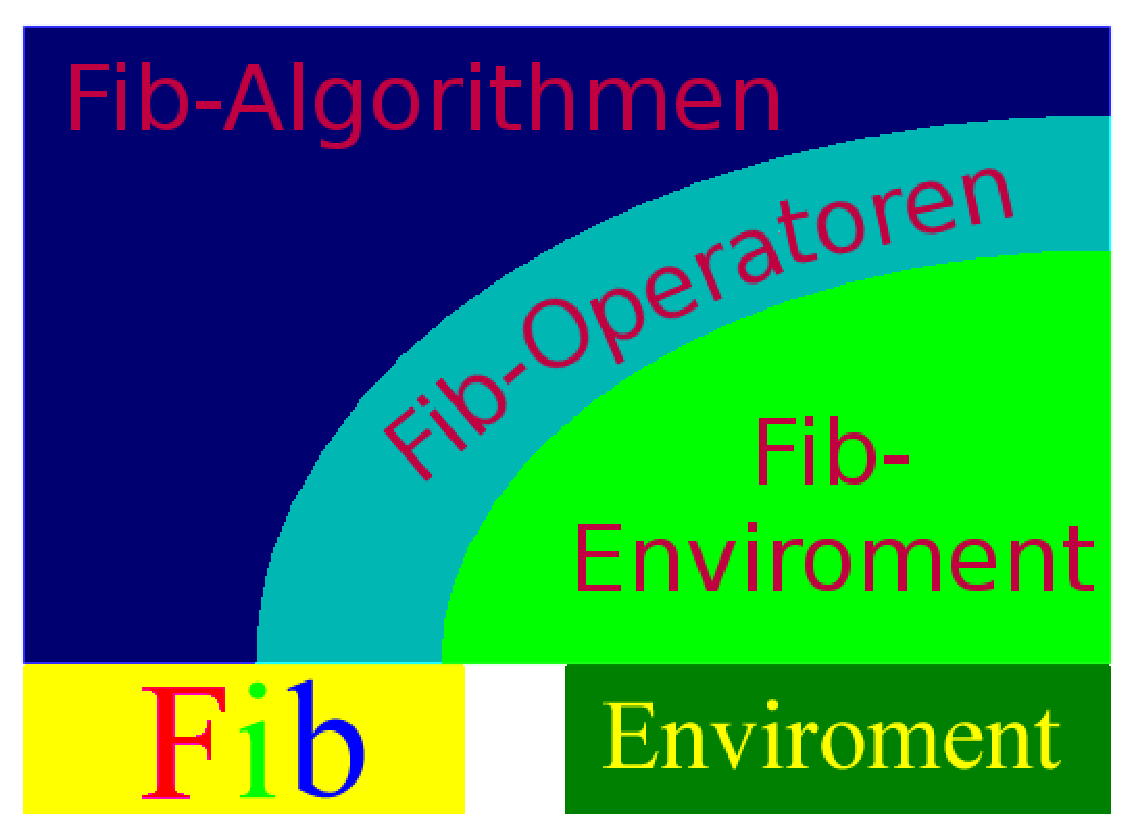
\includegraphics[scale=0.5]{ProjektAbhaengigkeiten}
\end{center}
\caption{Abh"angigkeiten der Hauptmodule}
\label{figMainModulDependencies}
\end{figure}

Das ``enviroment.fib'' Modul ben"otigt zwar f"ur seine Individuen die Fib-Objekte, dies jedoch nur als Namen (f"ur Fib-Objekte). Das ``enviroment.fib''-Modul ben"otigt also nur einen Namen f"ur Fib-Objekte und kein Wissen "uber die Funktionsweise (Methoden) der Fib-Objekte. Daher ist dass ``enviroment.fib''-Modul nicht von ``fib''-Modul abh"angig.















